\chapter{Introduction}
\label{chap:intro}
Robot controllers, and locomotion controllers in particular, can consist of many expert designed heuristics, for example feedback control of the Center of Mass (CoM) position and velocity, feedback control of robot joints, and designing reference trajectories and desired position. State of the art works in walking robots featuring such heuristics include \cite{feng2015optimization}, \cite{kuindersma2016optimization} and \cite{hubicki2016walking}. These heuristics consist of sets of inter-dependent parameters, which can be hard to tune, especially in higher dimensions. In such cases, it is an art, rather than a science, to tune these parameters. 
This complexity motivates methods for learning parameters automatically. A simple approach is to learn in simulation and deploy on hardware. However, due to commonly encountered differences between simulation and hardware, such as modelling errors, performance in simulation often does not transfer to hardware. On the other hand, directly learning on hardware can require a prohibitively large number of experiments, making it nearly impossible to learn these controllers using traditional methods. This has led to a surge in interest in data-efficient learning techniques for robotics. 

One popular data-efficient method for learning controller parameters is Bayesian Optimization (BO). BO is a sample-efficient gradient-free black-box optimization method that has been applied to a wide range of robotics problems. For example, \cite{Calandra2016}, \cite{marco2017virtual}, \cite{cully2015robots} try to learn parameters directly on hardware using BO. However, the performance of BO degrades in high dimensions (see~\cite{localBO17} for a related discussion), even for dimensionalities commonly encountered in locomotion controllers. We aim to overcome this problem by incorporating domain knowledge into BO.
\begin{figure}
    \centering
    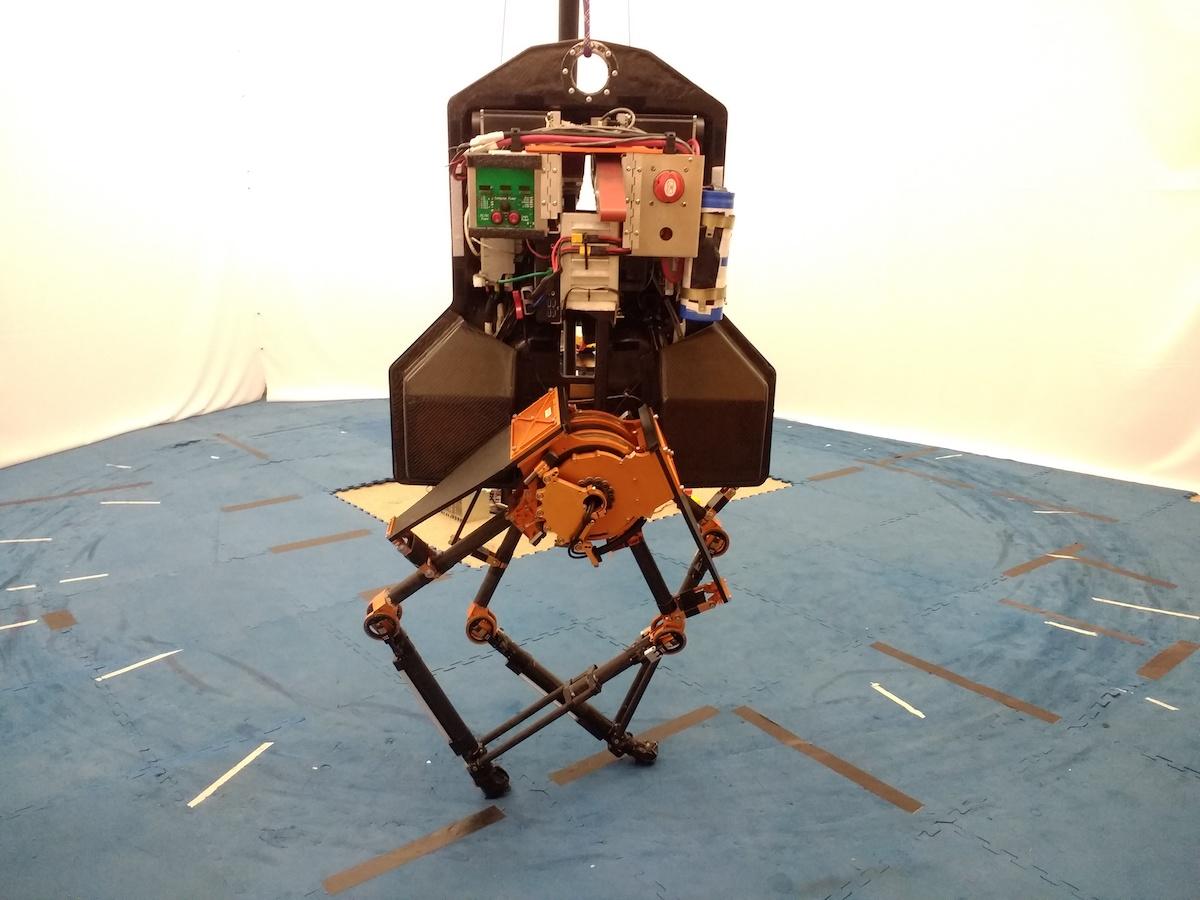
\includegraphics[width = 0.4\textwidth]{img/atrias1.jpg}
    %\includegraphics[width = 0.35\textwidth]{img/atrias2.jpg}
    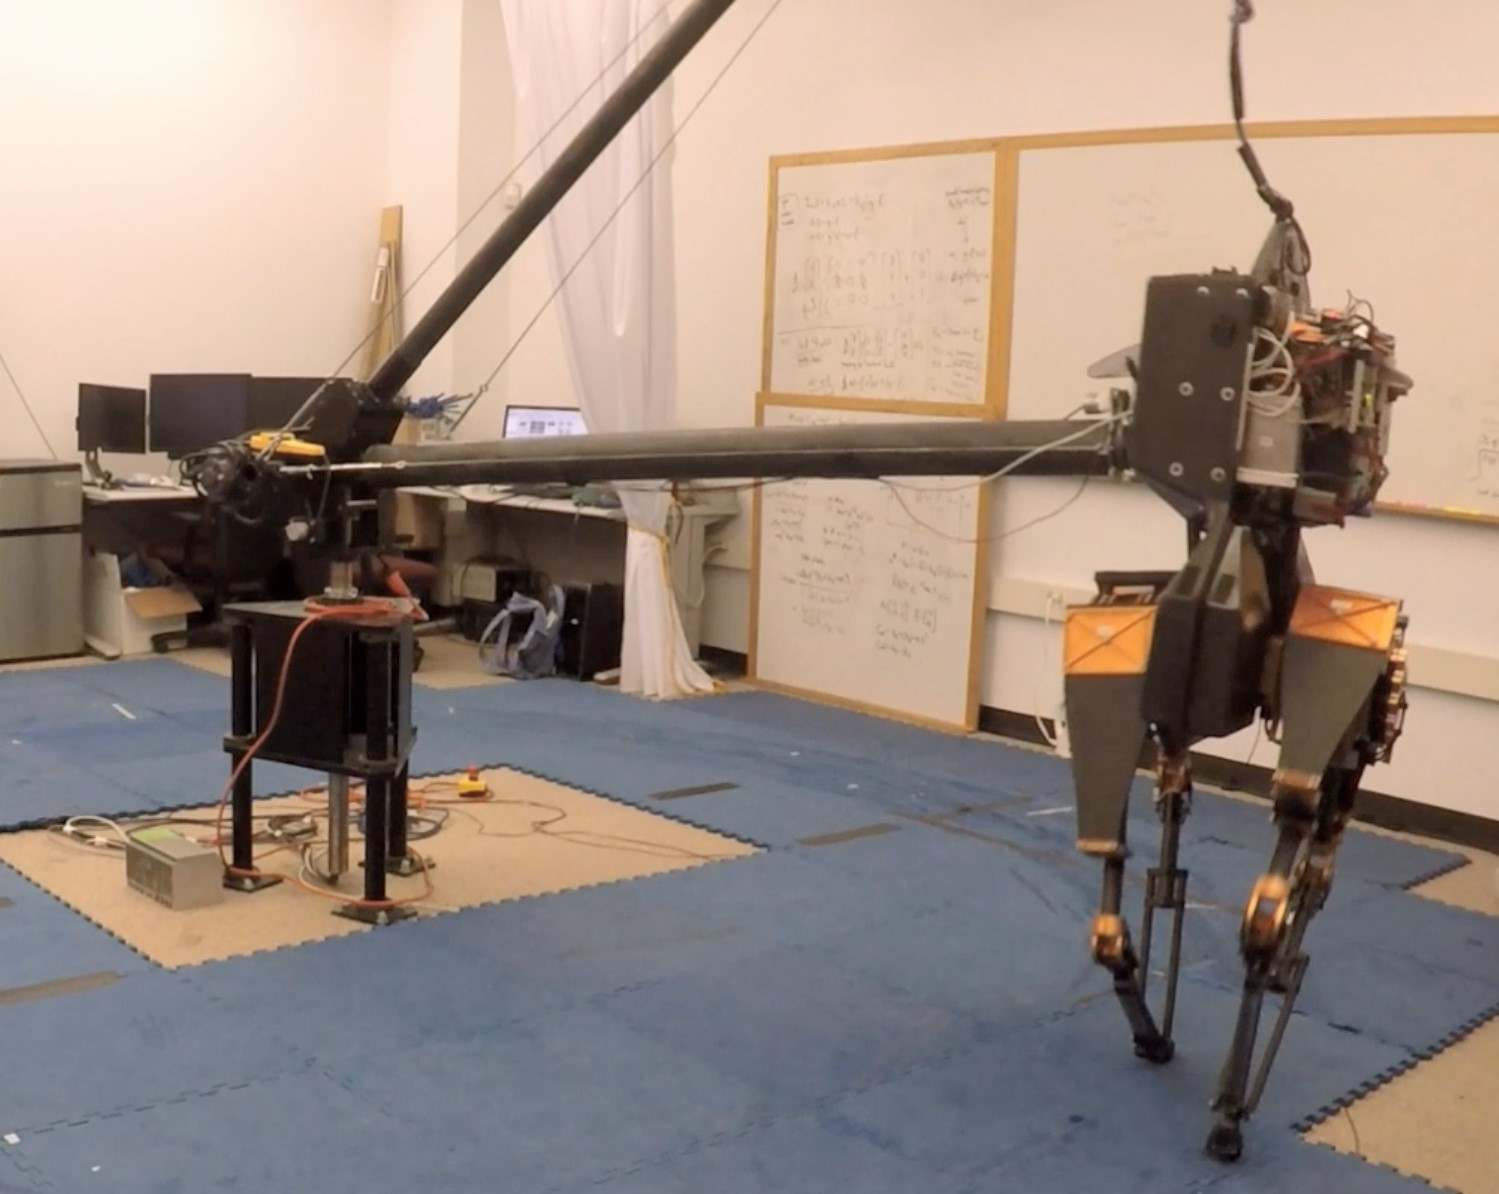
\includegraphics[width = 0.4\textwidth]{img/atrias_dog5d_walking_around_boom.jpg}
    \caption{\small{Our testbed is CMU's ATRIAS robot. 
    %While ATRIAS can walk in 3D, our experiments are focused on walking around a boom.
    }}
        \vspace{-5mm}
    \label{fig:atrias}
\end{figure}
%In our previous work, we proposed a transformation based on domain knowledge that reparameterized human-like walking controllers based on their behaviour in a high-fidelity simulation.
%The main idea was that some behavioural cues have a higher probability of transferring between simulation and hardware than exact cost or controller performance. For example, a controller that falls instantly in simulation by tilting its torso, would have a small chance of walking on hardware. On the other hand, a controller that walks efficiently in simulation might have a higher chance of walking on hardware, albeit with a different cost. Hence, it makes sense to roughly group parameters based on the behaviour they produce in simulation, and use this as a distance metric to distinguish between them. 

One way of incorporating domain knowledge could be to learn approximate models of the system from simulation, before moving to hardware. The idea of using simulation performance to speed up optimization on hardware has been explored before. A common approach is to learn controllers in simulation, and use this as a starting point on hardware. A domain expert would then typically have to fine-tune parameters on hardware. \cite{mordatch2015ensemble}~learn parameters using a collection of simulations that help account for model uncertainty. \cite{ha2015reducing}~iteratively learns both the model and controller parameters using the differences between simulated behaviors and observed hardware experiments. 
%\AR{Add work on developing transition models, model-based stuff here}
 \cite{marco2017virtual}~uses evaluations from simulation as a noisy prior for the optimization on hardware. \cite{cully2015robots}~pre-selects high performing controllers from simulation and search among them on hardware. 
 
\section{Adding prior knowledge to optimization}

 \textbf{We propose incorporating domain knowledge by building informed feature transforms that project the higher dimensional controller parameter space to an easy to optimize lower dimensional space of features.} These can be expert-designed or learned from data, as described below:
 
 \subsection{Expert-designed feature transforms}
 We use human-walking inspired features to develop a feature transform for bipedal walking that roughly groups controllers based on their walking features in short simulations. The objective of such a transformation is that some behavioural cues have a higher probability of transferring between simulation and hardware than exact cost or controller performance. For example, a controller that falls instantly in simulation by tilting its torso, would have a small chance of walking on hardware. On the other hand, a controller that walks efficiently in simulation might have a higher chance of walking on hardware, albeit with a different cost. Hence, it seems reasonable to roughly group parameters based on the behaviour they produce in simulation, and use this as a distance metric to distinguish between them. Despite being motivated by human walking features, these features also generalize to other robot morphologies and controllers, like the ATRIAS biped. 
 \subsection{Data-driven feature transforms}
Using extensive expert knowledge, as suggested above, has several advantages. It helps us learn and design features fast as well as provides transparency as to what the learning approach is prioritizing. However, it does raise concerns about problems for which such knowledge might not be available or as easily implementable. With this in mind, \textbf{we also develop a method to construct an informed metric automatically, without relying heavily on domain experts}. We propose to learn a distance metric with a neural network, utilizing data obtained from a high-fidelity simulator. This involves first running short simulations of a locomotion controller on a large grid of control parameters and recording the behavior of each set of parameters. The neural network then learns a mapping between input controller parameters and simulation output/behavior. We propose two ways of defining the target to be learned by the network. The first approach is based on the cost function that is to be optimized with BO on hardware, or a perturbed simulator. The second is cost-agnostic: learning to reconstruct a summary of robot trajectories obtained from simulation. This provides a useful re-parameterization: controller parameters that produce similar walking trajectory summaries are closer in this re-parameterized space. 
 
% Shall we name the controllers in the introduction: reactive and neuromuscular? Or is this to much detail for intro?

\section{Accounting for mismatch between hardware and simulation}
 An important question that arises when using simulation to guide hardware searches is: how can we learn and take into account the differences between simulation and hardware? For example \cite{macalpine2016adaptation} adapts the target task based on the mismatch between the expected and actual performance. \cite{marco2017virtual} develops an automatic way of transitioning between simulation and hardware based on data collected so far. 
 
 \textbf{We propose to learn a mismatch-map that represents the mismatch between behaviour encountered in simulation and hardware.} This allows us to build an error map over our parameter space, based on data. We start by trusting all simulation points with predicted mismatch of 0, and as we sample points on hardware, we update our estimate of error on each simulation sample. The advantage of this is that we can have different error values for different regions of parameter space, as some parts of the parameter space might transfer well between hardware and simulation, while others might not. %Using this trust-map, we can achieve significant sample-efficiency even with significantly perturbed simulations. %This is a promising result that is being tested on hardware.
To study the efficacy of this approach, we create a series of increasingly approximate simulators and use features from approximate simulators to optimize controllers on the original simulator. This allows us to empirically examine the deterioration of sample-efficiency as the simulator becomes more and more inaccurate, as well as the advantage of building a mismatch-map to close the loop between simulation and hardware. Our experiments show that this approach can learn controllers when simulation dynamics are perturbed by up to 60\% of their ``true" value. In addition, it is also robust to systematic under-modelling errors, such as unmodelled joint friction, actuator dynamics and other robot components. In comparison, other approaches from the literature that use simulation to speed up hardware experiments, such as \cite{cully2015robots}, suffer when simulation is significantly different from hardware. 

\AR{TODO : Implement 50d with mismatch on hardware}

\section{Using neural networks to learn walking policies}

While expert-designed policies are extremely powerful tools for sample-efficiency as well as safety of the robot, it can be challenging to design them in some situations. In such cases, high-dimensional policies like neural networks can be very useful. Typically, these are trained in simulation with deep reinforcement learning, and are shown to be capable of generating very diverse sets of behaviours. For example, \cite{silver2016mastering} use deep reinforcement learning to solve compledx long horizon games like AlphaGo, starting with no human input. Similar progress has been achieved in the domain of continuous control, dealing with very high dimensional state and action spaces. For example, Deep Deterministic Policy Gradients (DDPG) ~\cite{lillicrap2015continuous} and Trust Region Policy Optimization  (TRPO) ~\cite{schulman2015trust} can solve several control challenges in the Mujoco simulation environment \cite{todorov2012mujoco}. %\cite{heess2017emergence} show that a variant of the Proximal Policy Optimization (PPO) \cite{schulman2017proximal} can learn to control a very high degree of freedom humanoid robot in Mujoco, even in very challenging environments. Similarly, \cite{rajeswaran2017towards} use a variant of DDPG to learn to do dexterous manipulation with a high degree of freedom hand in simulation.

While simulation results for deep RL are very impressive, the simulation-hardware gap makes most controllers learned in simulation unsuitable to be implemented on hardware. This is partly because simulations are not perfect representations of real systems, but also because learning approaches often tend to exploit simulation inaccuracies to achieve better performance. 
%Recent work learns parameters of expert controllers on hardware sample-efficiently, for example \cite{antonova2017deep} and \cite{cully2015robots} use Bayesian Optimization. While these are promising, and robust even to hardware damage, they are limited by the controllers they can represent. On the other hand, high-dimensional neural network policies can approximate arbitrarily complex controllers, but too expensive to optimize on hardware. 
One approach to learn policies in simulation and deploy on hardware is domain randomization \cite{mordatch2015ensemble}. It can be used to learn robust neural network policies in simulation by applying random perturbations to the dynamics and other properties of the simulator. This approach has been applied to manipulation problems \cite{peng2017sim}, as well as quadrupedal locomotion problems \cite{tan2018sim}. However, typical domain randomization can lead to controllers that perform worse than controllers trained without randomization \citep{tan2018sim}, as well as make the learning problem much harder \citep{2018arXiv180800177O} taking over 100 years of simulation time to learn successful policies.   

 Domain randomization from scratch is especially challenging for under-actuated bipedal robots, as the basin of stability around a controller is typically very small. As a result, it is very difficult to randomly explore the space of controllers to find successful controllers that stabilize a wide range of dynamic models, and other disturbances. Moreover, the learned controllers would typically be quasi-static in nature, similar to \cite{mordatch2015ensemble} in behavior, which is not very impressive in performance. 
 
We experiment with classical deep reinforcement learning techniques to learn robust controllers in simulation and test them on hardware. Instead of using domain randomization, we create disturbances in simulation by simulating ground height disturbances and study the effect of policy structure on the rate of transfer. Starting with a high-fidelity simulator \citep{martin2015robust}, we experiment with different controller structures, and study their effect on transfer from simulation to hardware, without any domain randomization. The first neural network policy is a general policy that directly outputs the desired actions of the robot, while the second has the structure of an expert-designed policy and predicts the desired states for this policy. We find that structured neural network controllers have a fast training rate in simulation as well as higher rate of transfer to hardware. The structure also gives the user the power to modify the controller, if required, without having to re-train the neural network from scratch.


%Using our feature transform, we incorporate domain knowledge in BO, and optimize three walking controllers on ATRIAS - two on hardware and all three in simulation. BO equipped with domain knowledge is found to be much more sample-efficient than traditional BO. Using our trust-map, we can further improve sample-efficiency in perturbed simulation experiments. This is a promising result that needs to be tested on hardware in the future.
\section{Summary of completed goals and contributions}

In work done, we present evaluations of our proposed methods on the ATRIAS biped robot (Figure \ref{fig:atrias}), ATRIAS simulation, and a 7-link biped simulation. 

First, we use expert designed controllers and optimize their parameters using BO. We evaluate different feature transforms on three  controllers of increasing dimensionality. We start with a 5 dimensional feedback-based reactively stepping controller, and increase its dimensionality to 9. Then we take a 50-dimensional highly non-linear neuromuscular controller and optimize its parameters. We successfully optimize parameters for a 5-dimensional and 9-dimensional controller on the ATRIAS hardware in less than 10 trials, which proves to be challenging for traditional BO. Our results show that these feature transforms - hand-designed and data-driven, extract useful information from simulations, and leads to an effective transfer of knowledge to hardware. 
%This motivates future work for using our approach on hardware for the 50-dimensional controller.

While, Bayesian Optimization benefits from feature transforms and informed distance metrics, we also explore if simulation can be useful in learning other walking policies which might be much higher dimensional. We train two neural network policies - with and without structure and study their rate of transfer to hardware. Our studies show that structured neural network policies have a higher rate of transfer between simulation and hardware as compared to unstructured neural network polices.

The main contributions of this thesis are as below:
\begin{itemize}
    \item A simulation-based feature transform that enables faster optimization of bipedal walking controllers on hardware.
    \item A hybrid optimization approach that integrates model-based information from simulation into a model-free global search framework like Bayesian Optimization
    \item A novel way of updating models from hardware data using feature transforms evaluated on simulation and hardware
    \item A study of the effect of structure on neural network policies trained in simulation and their rate of transfer to hardware
\end{itemize}
%The rest of the paper is organized as follows: In Section \ref{sec:background} we present background on the concepts used in this paper and summarize related work. In Section \ref{sec:dog} we describe our approach of using a locomotion feature transform in detail. Section \ref{sec:atrias_cont} describes our test platform ATRIAS and the controllers used in our experiments. In Section \ref{sec:experiments} we describe our simulation and hardware experiments. Section \ref{sec:conclusions} concludes with further discussion.
